\section{Motores de juegos}
Un motor de juego es un framework software que facilita el desarrollo de videojuegos proveyendo  funcionalidad general necesaria para cualquier juego, como renderizado, físicas o lectura de entrada\cite{game_engine}.

Este termino surgió en la década de los noventa con juegos como Doom (Id Software, 1993), Quake (Id Software, 1996) o Unreal (Epic Games, 1998). Estos juegos habían sido desarrollados con una clara separación entre sus componentes software y resto de los assets del juego como el arte, los mapas de juego o las reglas; lo que permitía, con relativamente poco esfuerzo, crear juegos nuevos a partir de estos, siempre que tuviesen unas mecánicas de juego similares. El incremento en los últimos años del coste de la producción de los videojuegos ha producido que se generalice el uso de motores de jugo desarrollados por terceros. 

La principal diferencia entre los motores de juego y otras herramientas similares como las librerías es su \textit(Arquitectura basada en datos), la cual consiste en almacenar los assets del juego en forma de archivos independientes que el motor pueda interpretar, utilizando la menor cantidad posible de código especifico. Muchos motores ofrecen también entornos de desarrollo integrados los cuales incluyen herramientas para facilitar el desarrollo como editores de niveles y terrenos, importadores de ficheros o sistemas de control de versiones y depuración.

A continuación, listaremos algunos de los motores actuales más usados por ladores:

\subsection{Unity3D}
Unity\footnote{https://unity3d.com/unity}, conocido popularmente como Unity3D, es un motor de juego con su propio Entorno de Desarrollo Integrado (IDE) lanzado en el año 2005 por la compañía Unity Technologies. El desarrollo de este motor comenzó en el año 2002, encabezado por los desarrolladores David Helgason, Joachim Ante y Nicholas Francis, con el objetivo de crear una tecnología accesible para desarrolladores novatos y estudios pequeños.
\begin{figure}[h]
	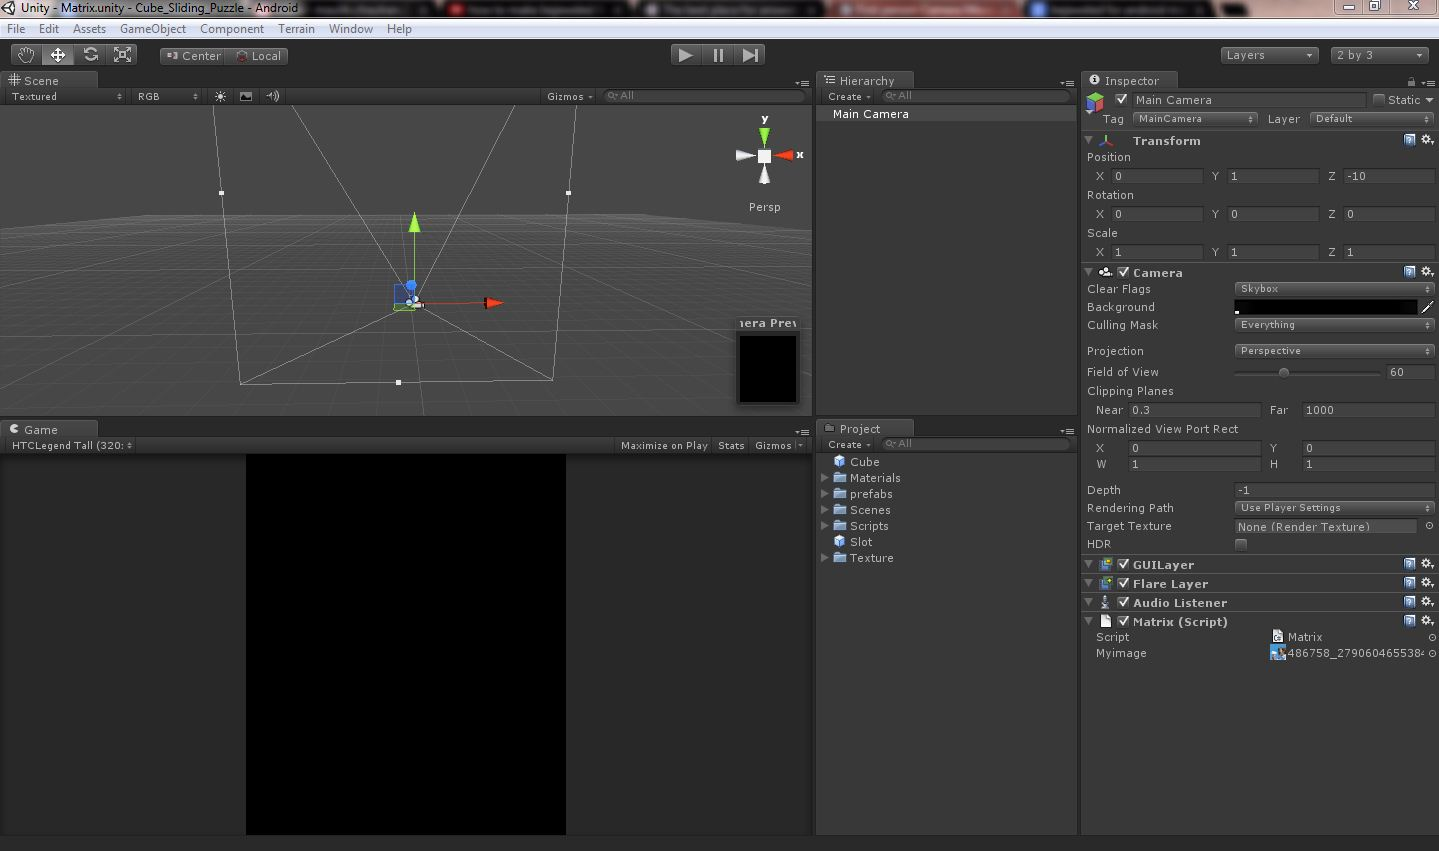
\includegraphics[width=0.8\textwidth]{images/estadodelarte/motores/captura-unity}
	\centering
	\caption{Captura del entorno de desarrollo}
\end{figure}

Unity cuenta con toda la tecnología necesaria para implementar un juego: Motor de renderizado en tiempo real, motor de físicas, sistemas de audio, sistemas de red... Sus puntos más fuertes son su facilidad de uso gracias a su editor gráfico personalizable, su facilidad para cargar recursos, su sistema de Scripting en C\#, su tienda virtual de recursos que ofrece un amplio abanico de material listo para usar y la posibilidad de exportación a multitud de plataformas (PC, Android, IOS, Consolas de sobremesa de diversas marcas...). Por otro lado, el rendimiento general de Unity es inferior al de otras propuestas similares, lo que reduce el alcance de los juegos que pueden ser desarrollados con él.

A la hora de adquirir el motor, Unity ofrece distintos planes de pago: La versión gratuita, Unity Personal, que ofrece la funcionalidad básica; Unity Plus que por 35€ al mes ofrece mayor personalización y herramientas de monetización; y la versión profesional, Unity Pro (125€ al mes), orientado a proyectos grandes.
\begin{figure}[!htb]
   \begin{minipage}{0.50\textwidth}
     \centering
     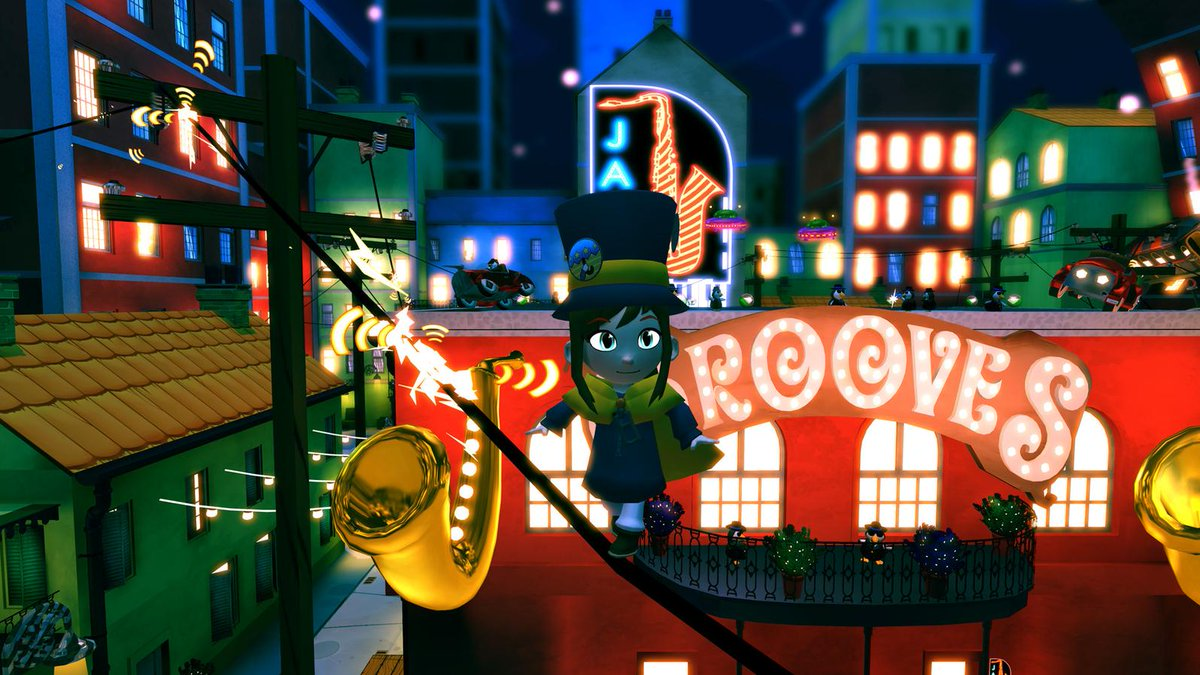
\includegraphics[width=0.9\linewidth, left]{images/estadodelarte/motores/hat-in-time}
     \caption{A Hat in Time (Gears for Breakfast, 2017)}
   \end{minipage}\hfill
   \begin {minipage}{0.50\textwidth}
     \centering
     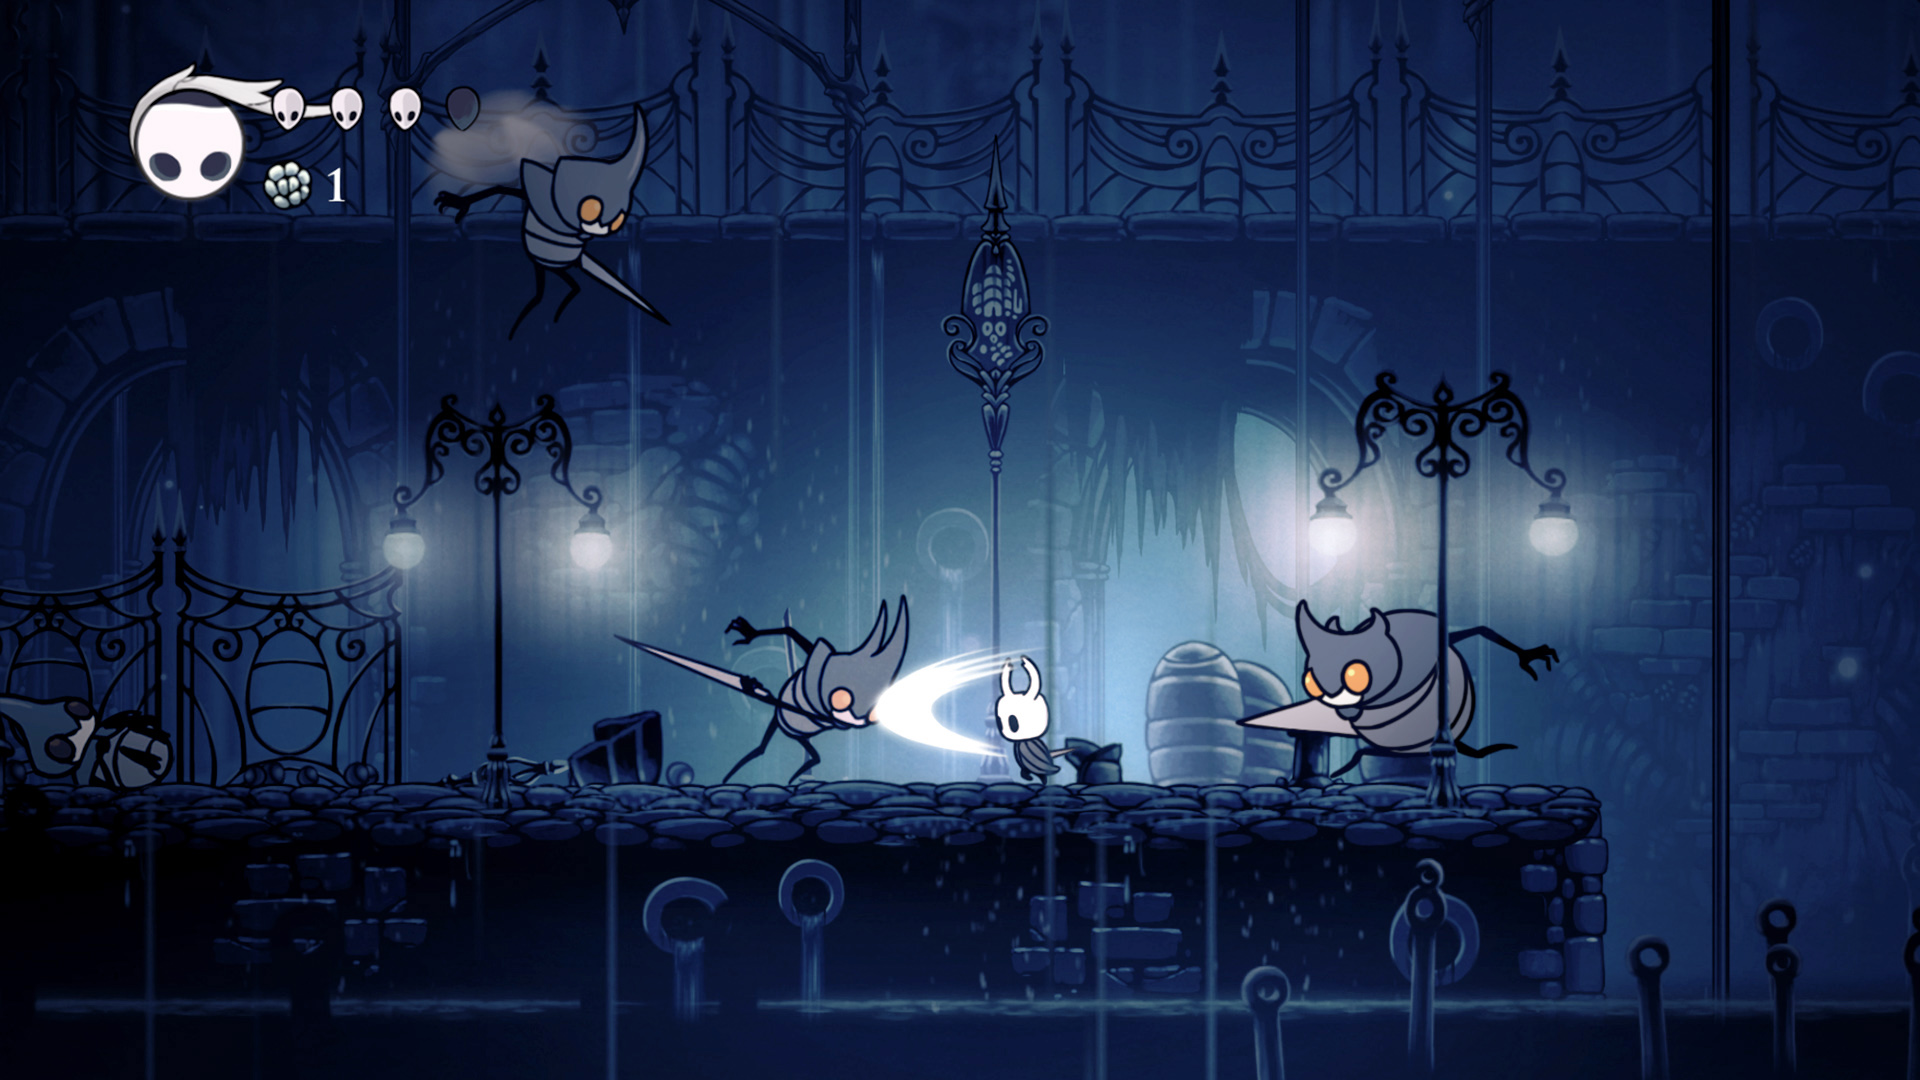
\includegraphics[width=0.9\linewidth, right]{images/estadodelarte/motores/hollow-knight}
     \caption{Hollow Knight (Team Cherry, 2017)}
   \end{minipage}
   \caption{Juegos desarrollados con Unity3D}
\end{figure}

\subsection{Unreal Engine}
El Unreal Engine\footnote{https://www.unrealengine.com/} es un popular motor de juego desarrollado por la compañía Epic Games. Originalmente desarrollado como motor propietario para el juego Unreal (1998), Epic Games pronto empezó a cerrar tratos con otras compañías que querían utilizar el motor en sus proyectos. Actualmente el motor se encuentra en su versión 4 y es uno de los más populares del sector, habiendo ganado incluso el premio Guinness al "motor de juegos más exitoso" con un total 408 juegos (a fecha de julio de 2014) desarrollados con Unreal. 
\begin{figure}[h]
	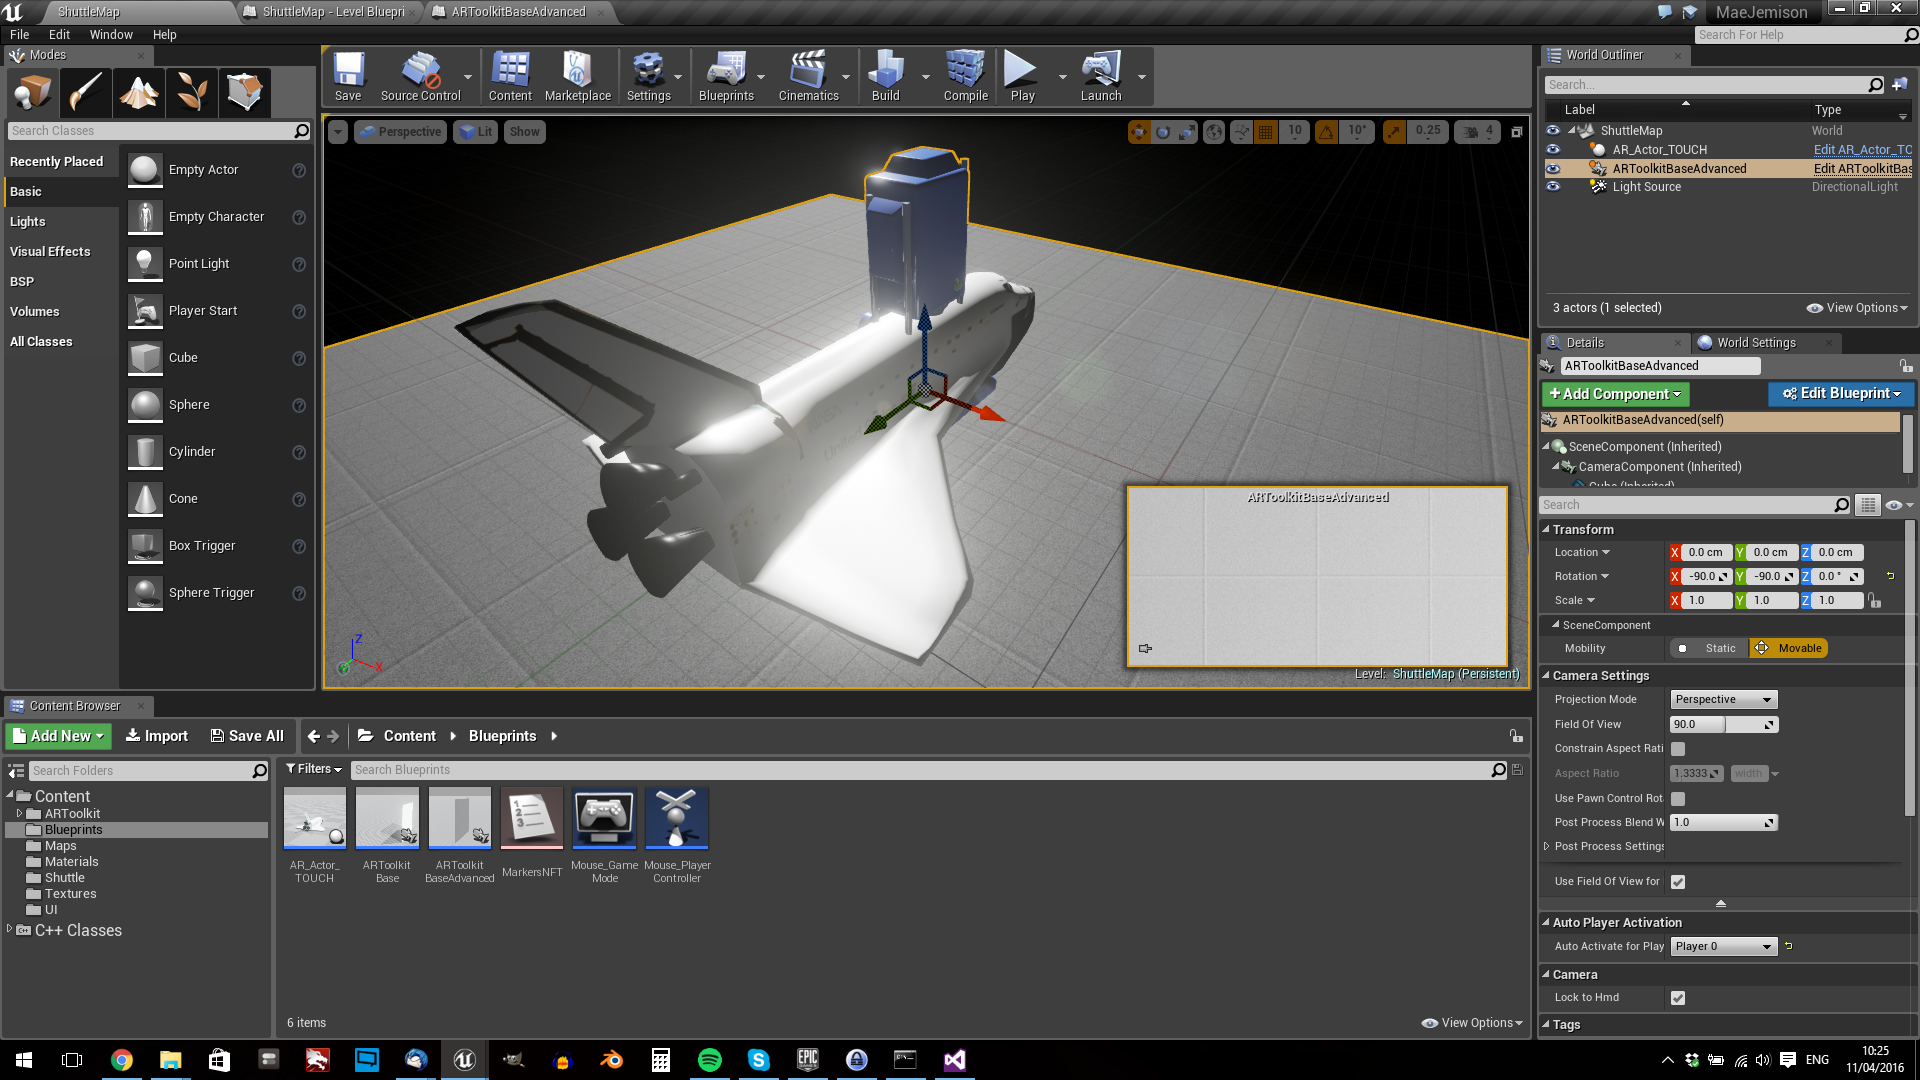
\includegraphics[width=0.8\textwidth]{images/estadodelarte/motores/captura-unreal}
	\centering
	\caption{Captura del entorno de Unreal Engine}
\end{figure}

Actualmente, Unreal Engine ofrece una suite completa de herramientas para el desarrollo de videojuegos y otras aplicaciones gráficas interactivas. El motor cuenta con un motor de renderizado fotorrealista, una robusta arquitectura para juegos en línea, el sistema Blueprint de programación gráfica y decenas de herramientas adicionales como generadores de terrenos, editor de materiales, etcétera. Unreal funciona íntegramente en C++, lo que permite exportar el proyecto a multitud de plataformas. Se trata por tanto de un motor orientado principalmente al desarrollo de juegos ``AAA'' llevados por equipos y compañías de gran envergadura, por lo que no resulta muy apropiado para proyectos pequeños. Por su diseño, el motor también se encuentra orientado al desarrollo de juegos de disparos en primera persona (FPS) por lo que desarrollar juegos de otros géneros, aunque no imposible, suponen una dificultad añadida.

Cuando un juego hace uso de Unreal Engine, un 5\% de los beneficios de este van a parar a Epic Games como compensación, pudiéndose negociar un pago por adelantado con la compañía en casos excepcionales.
\begin{figure}[!htb]
   \begin{minipage}{0.5\textwidth}
     \centering
     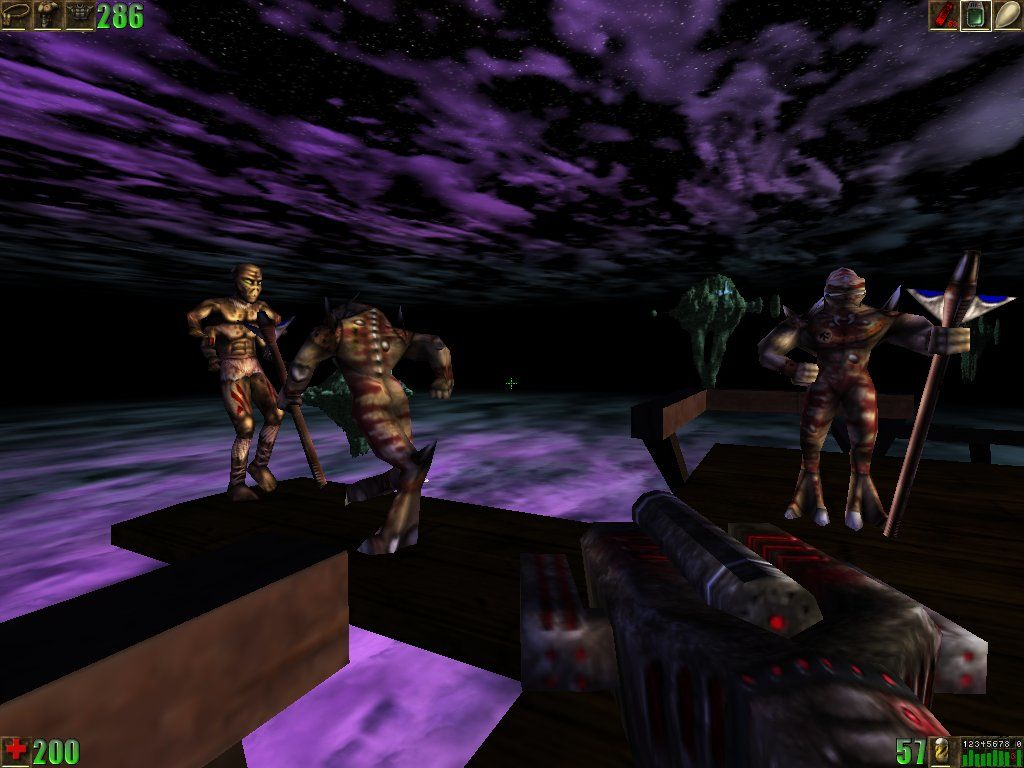
\includegraphics[width=0.85\linewidth, right]{images/estadodelarte/motores/unreal-original}
     \caption{Unreal (Epic Games, 1998)}
   \end{minipage}\hfill
   \begin {minipage}{0.5\textwidth}
     \centering
     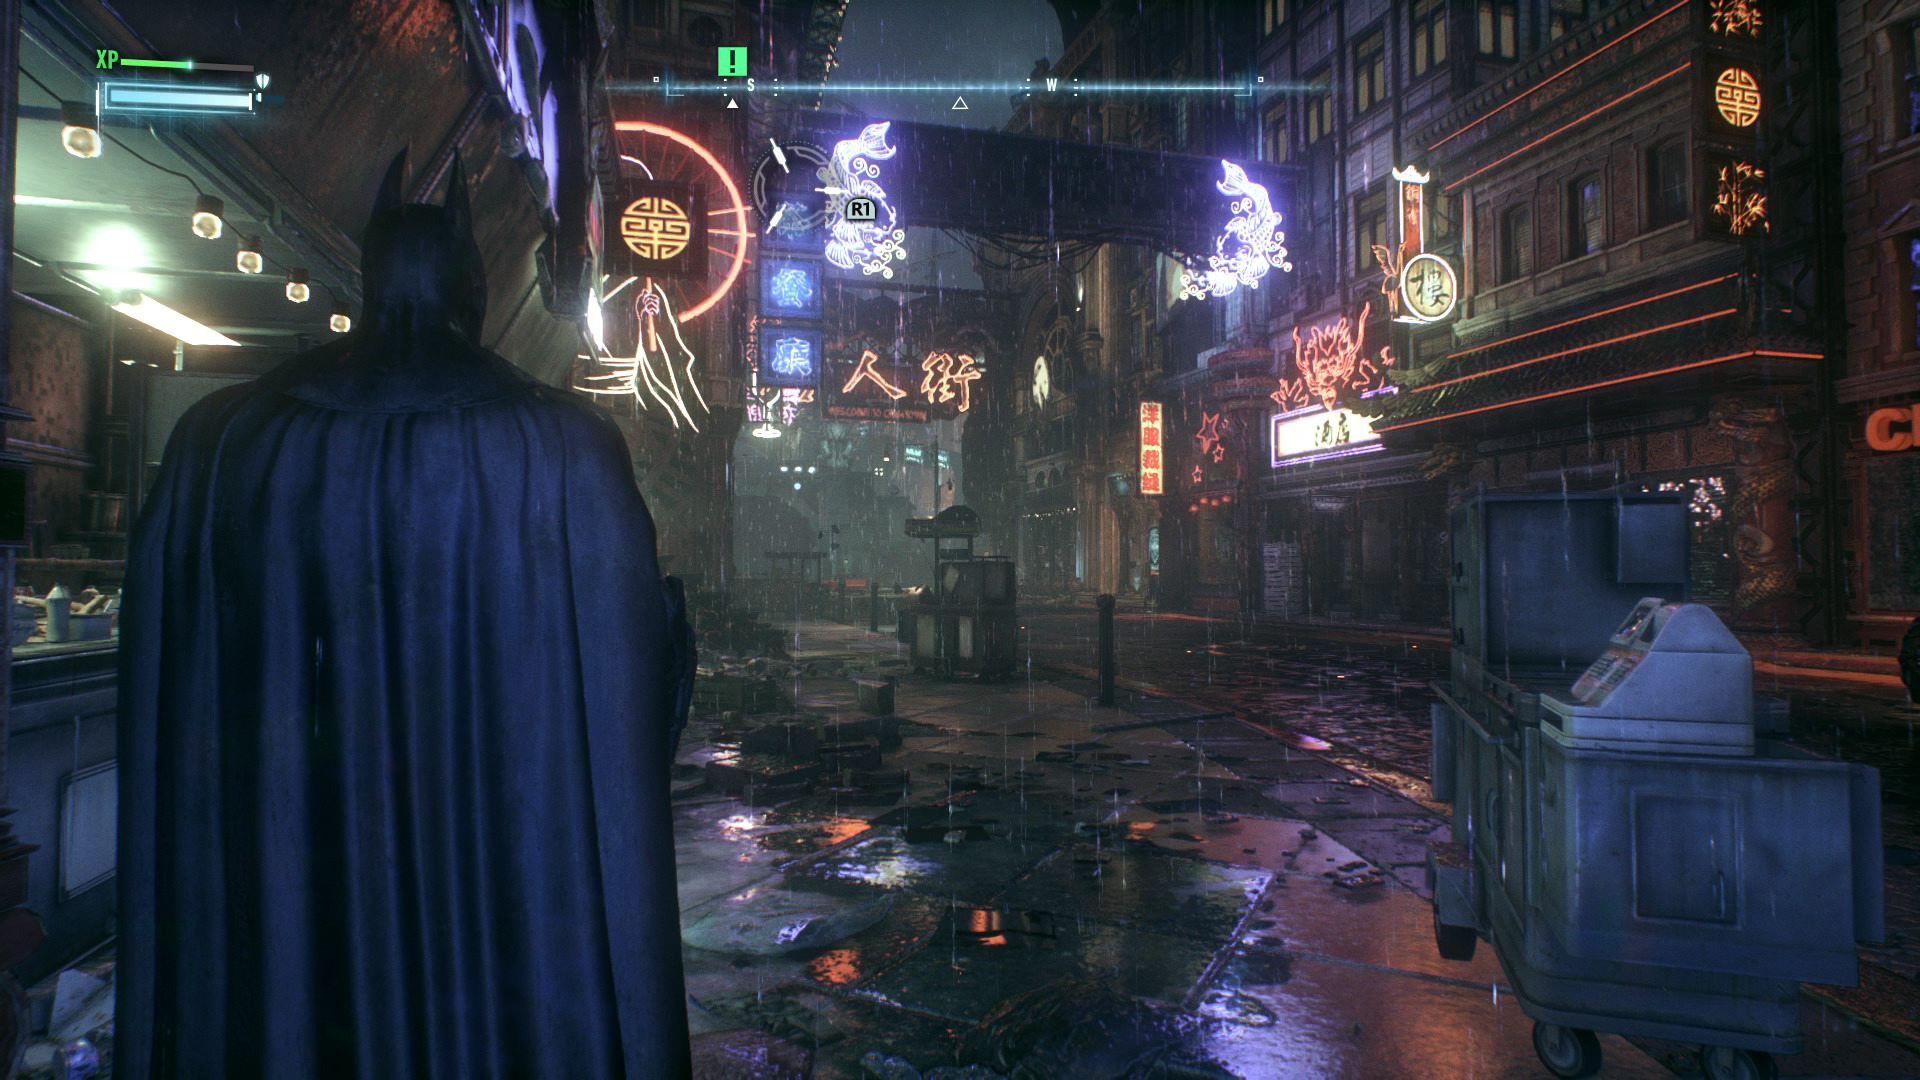
\includegraphics[width=0.85\linewidth, left]{images/estadodelarte/motores/batman-arkham}
     \caption{Batman: Arkham Knight (Rocksteady Studios, 2015)}
   \end{minipage}
   \caption{Juegos desarrollados con Unreal Engine}
\end{figure}

\subsection{Game Maker Studio}
Game Maker Studio\footnote{https://www.yoyogames.com/gamemaker} es un motor de juegos desarrollado por Yoyo Games. Su primera versión fue lanzada en el año 1999 y desde entonces ha evolucionado de una sencilla herramienta para crear juegos básicos para PC sin necesidad de conocimientos informáticos hasta convertirse en la suite de desarrollo profesional que es ahora.
\begin{figure}[h]
	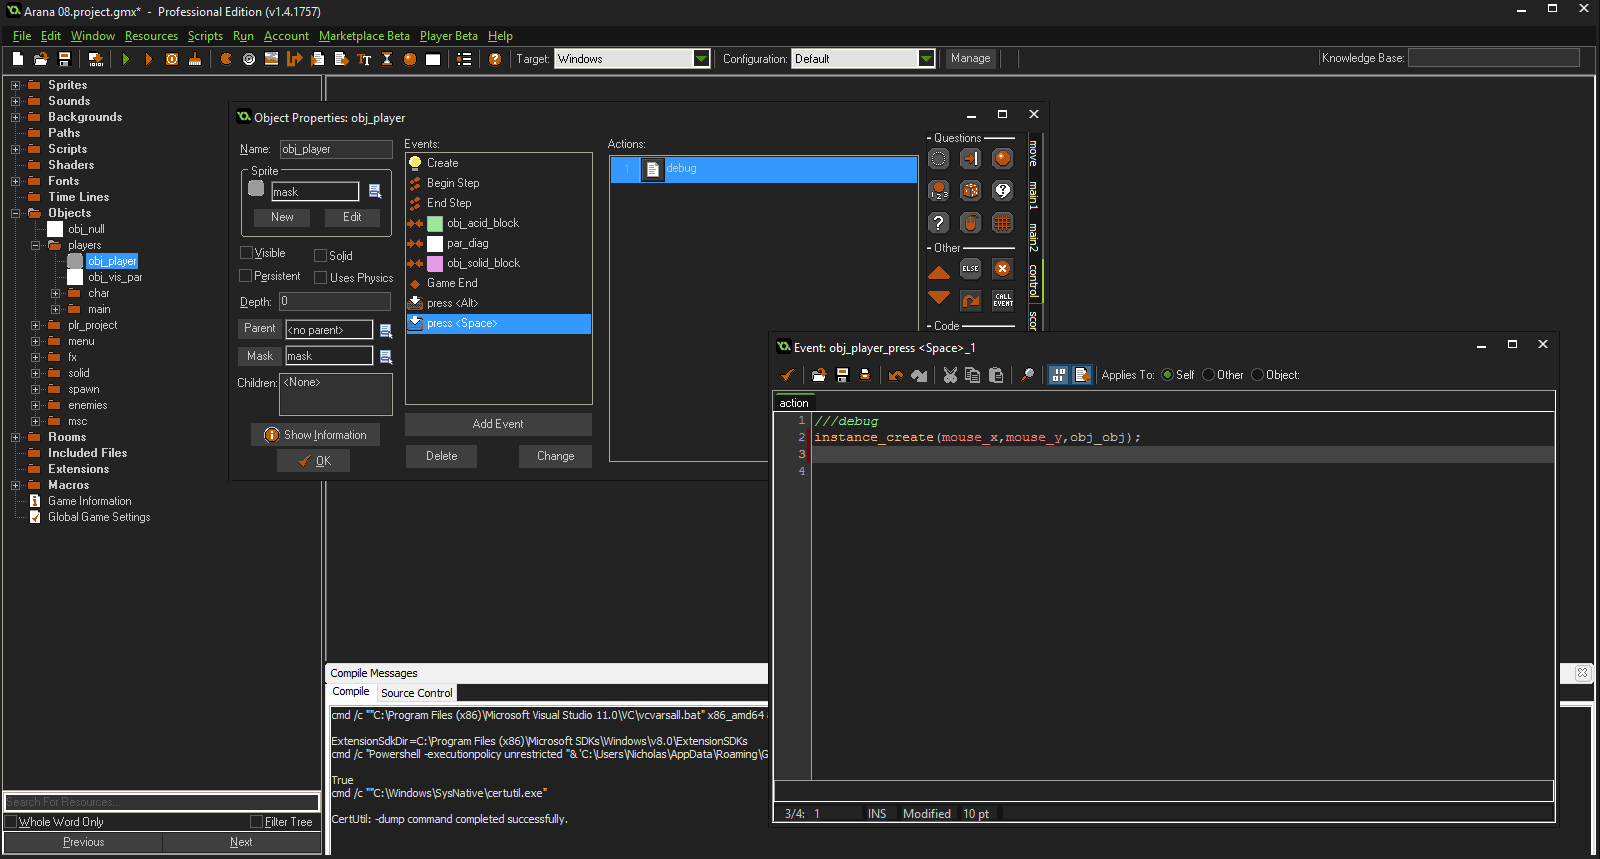
\includegraphics[width=0.8\textwidth]{images/estadodelarte/motores/captura-game-maker}
	\centering
	\caption{Captura del entorno de Game Maker Studio}
\end{figure}

El mayor punto fuerte de Game Maker es su sencillez a la hora de desarrollar juegos. La programación se realiza mediante el lenguaje de Scripting Game Maker Language o mediante su sistema "Drag and Drop" (arrastrar y soltar) lo que facilita enormemente el desarrollo. El entorno integrado incluye también herramientas complementarias como un editor gráfico y un editor de mapas para centralizar el desarrollo. Sin embargo, la sencillez del motor también se refleja en su potencia: Game Maker Studio está especialmente orientado a la producción de juegos sencillos y en 2D, por lo que no es apto para proyectos de gran envergadura o que requieran de gráficos tridimensionales elaborados.

La licencia de la versión actual de Game Maker Studio (Game Maker Studio 2) se encuentra a la venta por distintos precios dependiendo de la plataforma de distribución para la que se quiera trabajar: desde la versión básica por 39\$ anuales hasta la versión profesional permanente con posibilidad de exportación a IOS, Android y consolas por 399\$. Existen también una versión de prueba gratuita que cuenta con unas prestaciones reducidas y un plan de pago para su uso en centros educativos. 
\begin{figure}[!htb]
   \begin{minipage}{0.5\textwidth}
     \centering
     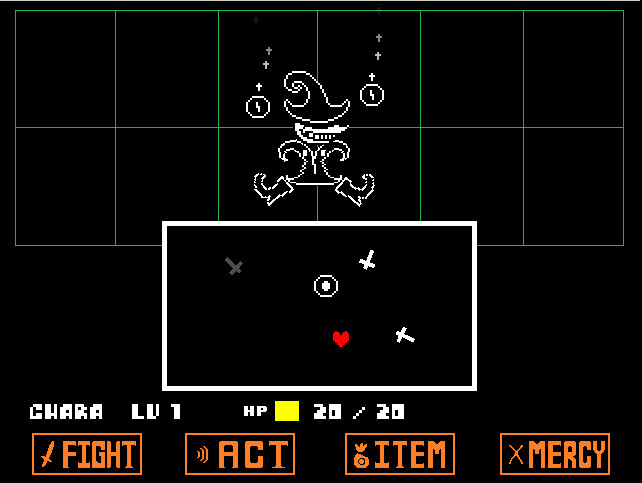
\includegraphics[width=0.85\linewidth, right]{images/estadodelarte/motores/undertale}
     \caption{Undertale (Toby Fox, 2015)}
   \end{minipage}\hfill
   \begin {minipage}{0.5\textwidth}
     \centering
     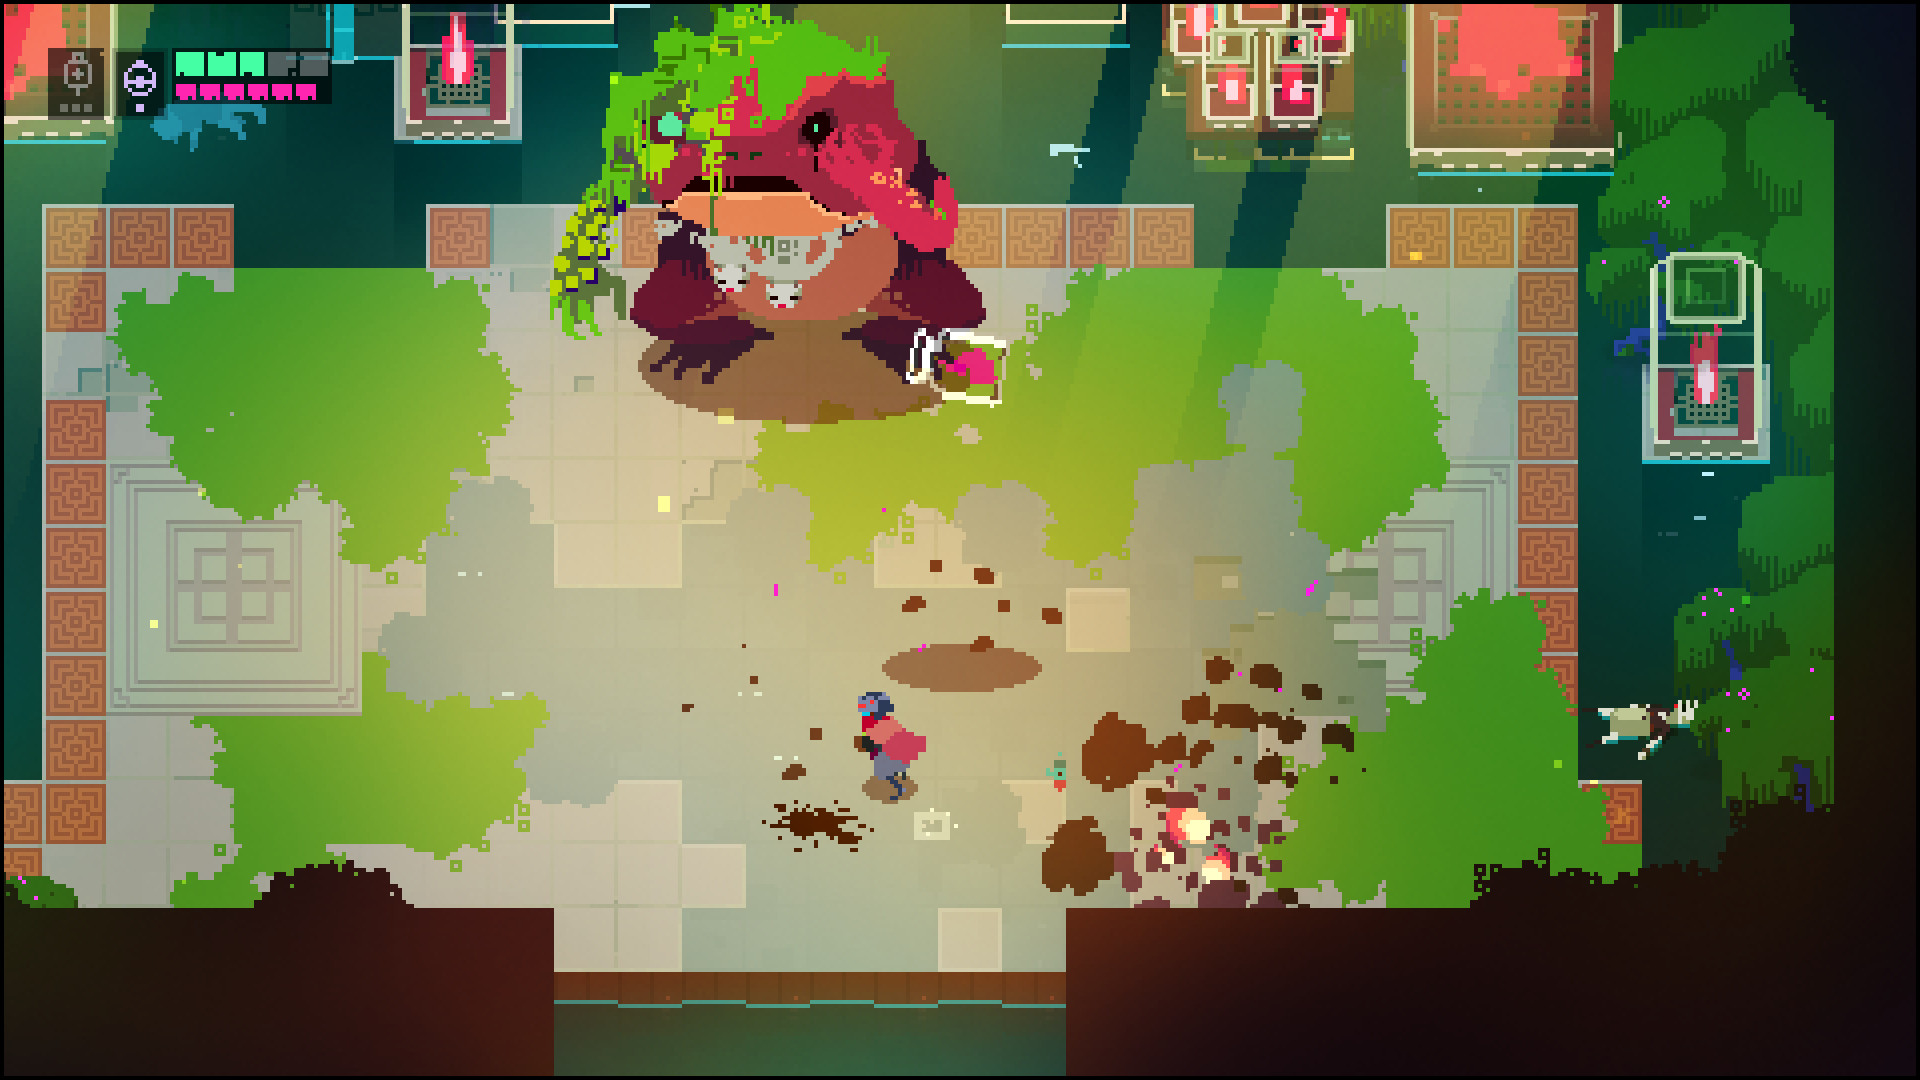
\includegraphics[width=0.85\linewidth, left]{images/estadodelarte/motores/hyper-light-drifter}
     \caption{Hyper Light Drifter (Heart Machine, 2016)}
   \end{minipage}
   \caption{Juegos desarrollados con Game Maker}
\end{figure}
